\documentclass[11pt]{article}

\title{Splitify}
\usepackage{graphicx}
\usepackage[utf8]{inputenc}
\usepackage{hyperref}
\usepackage{float}
\usepackage[left=2.5cm, right=2.5cm, top=2.5cm, bottom=2.5cm]{geometry}
\usepackage{titlesec}
\usepackage{tocloft} % Optional: to customize TOC appearance

% Redefine paragraph to behave like a subsection for TOC purposes
\titleformat{\paragraph}
  [runin] % Keep the paragraph style without line break
  {\normalfont\normalsize\bfseries} % Style
  {\theparagraph} % Numbering style
  {1em}
  {}

\titlespacing*{\paragraph}{0pt}{3.25ex plus 1ex minus .2ex}{1em}

\setcounter{secnumdepth}{4}
\setcounter{tocdepth}{4}
\author{Domingo Dirutigliano}


\begin{document}

\begin{titlepage}
   \begin{center}
       \vspace*{1cm}

       \LARGE{\textbf{Splitify Project}}

       \vspace{0.5cm}
        Documentazione generale

       \vspace{0.5cm}

       \begin{figure}[H]
    		\centering
    		
\includegraphics[width=0.2\textwidth]{assets/logo.png}
		\end{figure}

       \vspace{0.5cm}

       \textbf{Domingo Dirutigliano}

       \vfill

       \textbf{Politecnico di Bari}\\
       Fondamenti Web

       \vspace{0.1cm}
   \end{center}
\end{titlepage}

\tableofcontents
\newpage
\section{Scenario applicativo}
Splitify è un'applicazione web progettata per semplificare la gestione e la divisione delle spese tra gruppi di persone. Questo strumento è particolarmente utile per gestire spese condivise in contesti come viaggi, cene, eventi o convivenze, dove più persone contribuiscono finanziariamente e necessitano di un sistema per tenere traccia di chi ha pagato cosa e come dovrebbero essere suddivise le spese.

\subsection{Funzionalità principali}
L'applicazione Splitify offre le seguenti funzionalità principali:
\begin{itemize}
    \item Creazione e gestione di diverse \textit{board} (lavagne) per organizzare le spese per eventi o gruppi specifici
    \item Aggiunta di membri all'interno di una board, rappresentanti le persone coinvolte nelle spese
    \item Creazione di categorie per classificare le diverse tipologie di spese
    \item Registrazione di prodotti con relativi prezzi, associati a specifiche categorie
    \item Tracciamento delle transazioni finanziarie tra membri del gruppo
    \item Calcolo automatico dei saldi e delle somme dovute da ciascun membro
    \item Ottimizzazione dei rimborsi attraverso un algoritmo di backtracking che calcola la sequenza ottimale di transazioni per minimizzare il numero di scambi necessari
    \item Condivisione delle board con altri utenti con diversi livelli di permessi
\end{itemize}

\subsection{Architettura dell'applicazione}
Splitify è sviluppato come applicazione web full-stack seguendo un'architettura client-server:

\begin{itemize}
    \item \textbf{Frontend}: Implementato utilizzando React.js, TypeScript e Mantine UI per l'interfaccia utente. Il frontend comunica con il backend tramite chiamate API REST e connessioni WebSocket per gli aggiornamenti in tempo reale.
    \item \textbf{Backend}: Sviluppato utilizzando Node.js con il runtime Bun e TypeScript, fornisce API RESTful per la gestione dei dati e implementa logiche di business. Utilizza WebSocket per la comunicazione in tempo reale con il frontend.
    \item \textbf{Database}: MongoDB viene utilizzato come database NoSQL per la persistenza dei dati.
    \item \textbf{Autenticazione}: Il sistema utilizza autenticazione basata su JWT (JSON Web Token) per gestire sessioni e autorizzazioni degli utenti.
\end{itemize}

L'applicazione è containerizzata utilizzando Docker, facilitando il deployment in diversi ambienti e la configurazione del sistema.

\subsection{Sistema di autenticazione}
Splitify implementa un sistema di autenticazione robusto basato su token JWT (JSON Web Token):

\begin{itemize}
    \item \textbf{Autenticazione iniziale}: Quando un utente effettua il login con le proprie credenziali, il server verifica l'identità dell'utente e, se le credenziali sono valide, genera un JWT firmato contenente l'identificativo dell'utente e della sessione.

    \item \textbf{Struttura del token}: Il token JWT contiene informazioni essenziali nel payload come:
    \begin{itemize}
        \item \texttt{sub}: Identificativo dell'utente
        \item \texttt{sid}: Identificativo univoco della sessione
        \item \texttt{exp}: Timestamp di scadenza del token
        \item \texttt{iat}: Timestamp di emissione del token
    \end{itemize}

    \item \textbf{Gestione delle sessioni}: Il sistema tiene traccia delle sessioni attive dell'utente nel database, memorizzando per ciascuna sessione un identificativo univoco, la data di creazione, la data di scadenza e l'ultimo utilizzo.

    \item \textbf{Meccanismo di refresh}: Per migliorare la sicurezza senza compromettere l'esperienza utente, i token hanno una durata limitata. Quando un token sta per scadere, il client può richiamare l'endpoint \texttt{/token/refresh} per ottenere un nuovo token senza richiedere nuovamente le credenziali dell'utente. Questo meccanismo:
    \begin{itemize}
        \item Verifica che il token attuale sia ancora valido
        \item Controlla che la sessione corrispondente sia attiva nel database
        \item Aggiorna il timestamp di ultimo utilizzo della sessione
        \item Genera un nuovo token con una nuova scadenza estesa
    \end{itemize}

    Il refresh del token può essere effettuato solo nell'ultimo 20\% della sua durata totale. Il frontend implementa un sistema intelligente di refresh che, decodificando il token JWT, calcola automaticamente quando è necessario rinnovarlo e richiama l'endpoint di refresh in modo asincrono nell'ultimo 9\% della durata del token, evitando così interruzioni dell'esperienza utente o ricaricamenti della pagina.

    \item \textbf{Opzione "mantieni accesso"}: Durante il login, l'utente può scegliere l'opzione "mantieni accesso" (\texttt{keepLogin}), che estende significativamente la durata della sessione memorizzata nel database, permettendo refresh del token per periodi più lunghi.

    \item \textbf{Gestione delle sessioni multiple}: Il sistema supporta fino a un massimo di 10 sessioni attive contemporaneamente per ciascun utente. Quando viene raggiunto questo limite e l'utente effettua un nuovo login, la sessione più vecchia viene automaticamente invalidata. L'utente può inoltre invalidare tutte le sessioni attive semplicemente cambiando la propria password.
\end{itemize}

Ogni richiesta API che richiede autenticazione include il token JWT nell'header di autorizzazione. Un middleware del backend verifica la validità del token prima di permettere l'accesso alle risorse protette.

\section{Diagrammi UML}

\subsection{Diagramma dei casi d'uso}
Il diagramma dei casi d'uso illustra le interazioni tra gli attori del sistema (utenti non autenticati, utenti registrati e amministratori) e le funzionalità offerte dall'applicazione.

\begin{figure}[H]
    \centering
    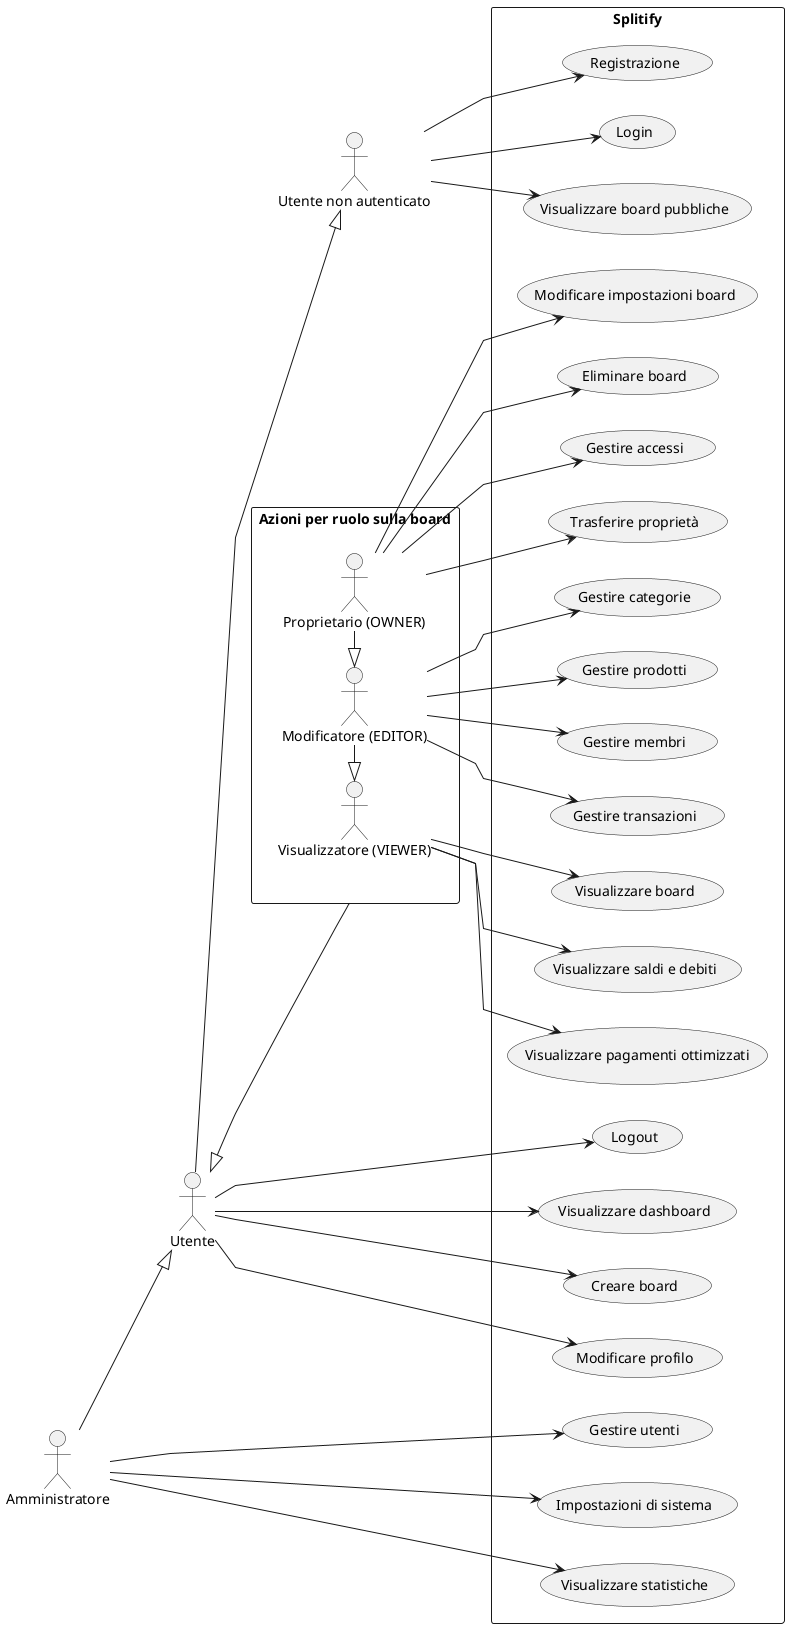
\includegraphics[width=0.5\textwidth]{assets/usecase.png}
    \caption{Diagramma dei casi d'uso di Splitify}
\end{figure}

Gli attori principali sono:
\begin{itemize}
    \item \textbf{Utente non autenticato}: può registrarsi al sistema o effettuare il login. Inoltre, ha la possibilità di visualizzare le board che sono state impostate come pubbliche, anche senza autenticazione.
    \item \textbf{Utente}: dopo l'autenticazione, può gestire board, categorie, prodotti, membri e transazioni, oltre a poter modificare il proprio profilo.
    \item \textbf{Amministratore}: oltre a tutte le funzionalità dell'utente, ha accesso alle funzionalità di amministrazione come la gestione degli utenti, le impostazioni di sistema e la visualizzazione delle statistiche.
\end{itemize}

\subsection{Modello dei dati}
Il seguente diagramma mostra il modello dei dati utilizzato in Splitify, rappresentando le entità principali e le loro relazioni:

\begin{figure}[H]
    \centering
    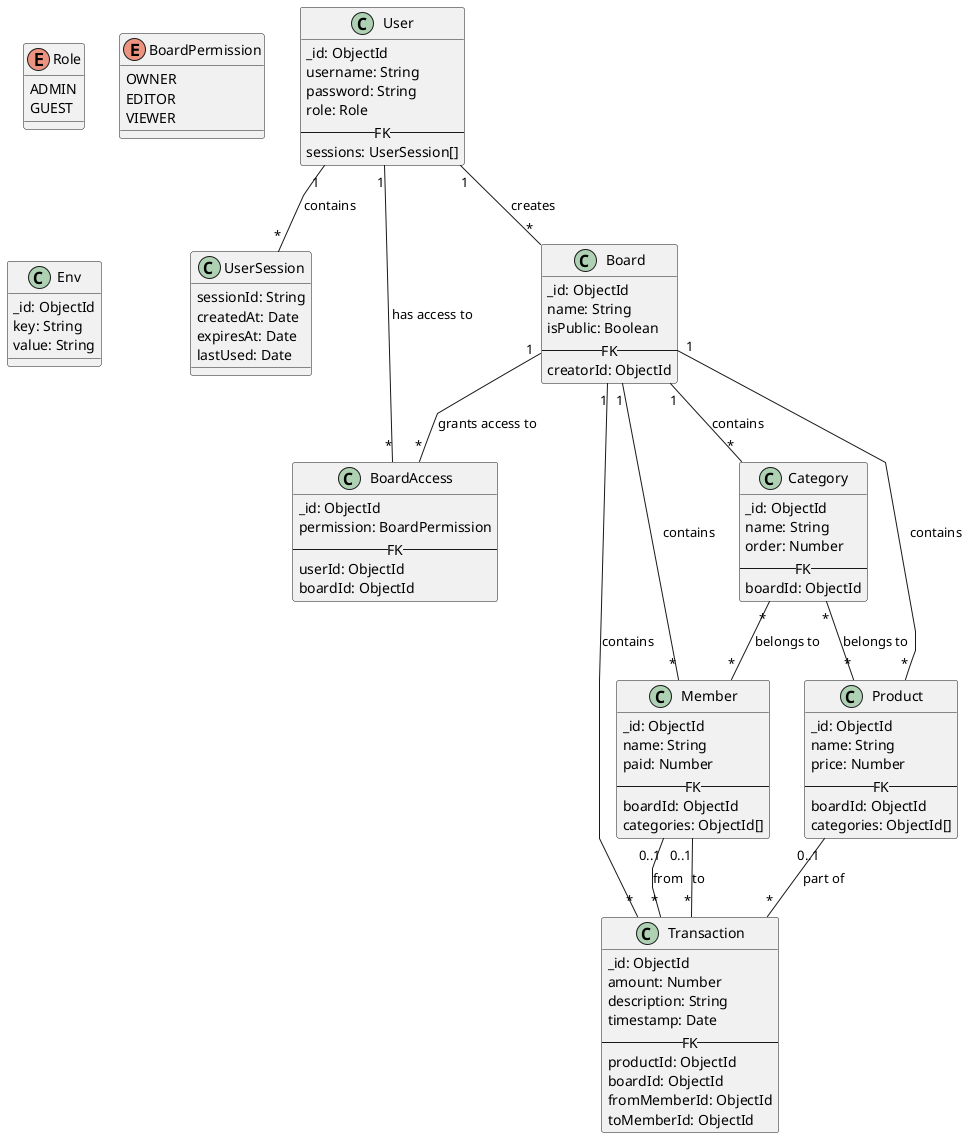
\includegraphics[width=0.75\textwidth]{assets/dbmodel.png}
    \caption{Modello dei dati di Splitify}
\end{figure}

\section{Modello dei dati}

Nel diagramma ER sono state volutamente inserite le chiavi esterne anche se normalmente, nella rappresentazione Entity-Relationship pura, queste non andrebbero incluse. Questa scelta è stata fatta per evidenziare esplicitamente come sono state implementate le associazioni tra le entità in MongoDB, un database NoSQL. Il modello dei dati non segue la normalizzazione tipica dei database relazionali, ma è strutturato secondo il paradigma document-oriented di MongoDB, dove i riferimenti tra documenti vengono implementati tramite campi che contengono gli identificatori (ObjectId) di altri documenti.
Il modello dei dati di Splitify è composto dalle seguenti entità principali:

\subsection{User}
Rappresenta un utente registrato nel sistema.
\begin{itemize}
    \item \textbf{\_id}: Identificatore univoco (ObjectId)
    \item \textbf{username}: Nome utente univoco
    \item \textbf{password}: Password hashata
    \item \textbf{role}: Ruolo dell'utente (ADMIN o GUEST)
    \item \textbf{sessions}: Array di sessioni utente attive
\end{itemize}

\subsection{UserSession}
Rappresenta una sessione di autenticazione attiva.
\begin{itemize}
    \item \textbf{sessionId}: Identificatore univoco della sessione
    \item \textbf{createdAt}: Data e ora di creazione
    \item \textbf{expiresAt}: Data e ora di scadenza
    \item \textbf{lastUsed}: Data e ora dell'ultimo utilizzo
\end{itemize}

\subsection{Board}
Rappresenta una lavagna di gestione spese.
\begin{itemize}
    \item \textbf{\_id}: Identificatore univoco (ObjectId)
    \item \textbf{name}: Nome della board
    \item \textbf{isPublic}: Flag che indica se la board è pubblica
    \item \textbf{creatorId}: Riferimento all'utente creatore (ObjectId)
\end{itemize}

\subsection{BoardAccess}
Gestisce i permessi di accesso alle board per gli utenti.
\begin{itemize}
    \item \textbf{\_id}: Identificatore univoco (ObjectId)
    \item \textbf{userId}: Riferimento all'utente (ObjectId)
    \item \textbf{boardId}: Riferimento alla board (ObjectId)
    \item \textbf{permission}: Livello di permesso (OWNER, EDITOR, VIEWER)
\end{itemize}

\subsection{Category}
Rappresenta una categoria di spese.
\begin{itemize}
    \item \textbf{\_id}: Identificatore univoco (ObjectId)
    \item \textbf{boardId}: Riferimento alla board (ObjectId)
    \item \textbf{name}: Nome della categoria
    \item \textbf{order}: Ordine di visualizzazione
\end{itemize}

\subsection{Member}
Rappresenta un membro partecipante alla divisione delle spese.
\begin{itemize}
    \item \textbf{\_id}: Identificatore univoco (ObjectId)
    \item \textbf{boardId}: Riferimento alla board (ObjectId)
    \item \textbf{name}: Nome del membro
    \item \textbf{paid}: Importo pagato
    \item \textbf{categories}: Array di riferimenti a categorie (ObjectId[])
\end{itemize}

\subsection{Product}
Rappresenta un prodotto o servizio acquistato.
\begin{itemize}
    \item \textbf{\_id}: Identificatore univoco (ObjectId)
    \item \textbf{boardId}: Riferimento alla board (ObjectId)
    \item \textbf{name}: Nome del prodotto
    \item \textbf{price}: Prezzo del prodotto
    \item \textbf{categories}: Array di riferimenti a categorie (ObjectId[])
\end{itemize}

\subsection{Transaction}
Rappresenta un movimento finanziario tra membri.
\begin{itemize}
    \item \textbf{\_id}: Identificatore univoco (ObjectId)
    \item \textbf{boardId}: Riferimento alla board (ObjectId)
    \item \textbf{fromMemberId}: Riferimento al membro pagante (ObjectId, opzionale)
    \item \textbf{toMemberId}: Riferimento al membro beneficiario (ObjectId, opzionale)
    \item \textbf{amount}: Importo della transazione
    \item \textbf{description}: Descrizione della transazione
    \item \textbf{productId}: Riferimento al prodotto associato (ObjectId, opzionale)
    \item \textbf{timestamp}: Data e ora della transazione
\end{itemize}

\subsection{Env}
Memorizza variabili di configurazione dell'ambiente.
\begin{itemize}
    \item \textbf{\_id}: Identificatore univoco (ObjectId)
    \item \textbf{key}: Nome della variabile
    \item \textbf{value}: Valore della variabile
\end{itemize}

\section{API Backend}
Il backend di Splitify espone una serie di API RESTful per interagire con il sistema. Le API sono organizzate nei seguenti gruppi:

\subsection{Autenticazione (/)}
\begin{itemize}
    \item \textbf{POST /login}: Autentica un utente e restituisce un token JWT. Accetta i parametri \texttt{username}, \texttt{password} e un flag opzionale \texttt{keepLogin} per mantenere la sessione attiva più a lungo.
    \item \textbf{GET /me}: Restituisce i dati dell'utente autenticato basandosi sul token JWT fornito nell'header di autorizzazione.
    \item \textbf{POST /register}: Registra un nuovo utente con username e password. La registrazione può essere aperta a tutti o richiedere un token, a seconda delle impostazioni del sistema.
    \item \textbf{POST /register/:token}: Registra un nuovo utente utilizzando un token di invito specifico, utile quando la registrazione è ristretta.
    \item \textbf{POST /token/refresh}: Rinnova il token di autenticazione generando un nuovo token JWT con una nuova data di scadenza, mantenendo la stessa sessione dell'utente.
    \item \textbf{GET /register/info}: Ottiene informazioni sulla modalità di registrazione attualmente configurata.
    \item \textbf{PUT /register/set}: Imposta la modalità di registrazione del sistema (aperta, chiusa o con token). Riservata agli amministratori.
\end{itemize}

\subsection{Gestione Board (/boards)}
\begin{itemize}
    \item \textbf{GET /boards}: Ottiene la lista delle board dell'utente
    \item \textbf{GET /boards/:id}: Ottiene i dettagli di una specifica board
    \item \textbf{POST /boards}: Crea una nuova board
    \item \textbf{PUT /boards/:id}: Aggiorna una board esistente
    \item \textbf{DELETE /boards/:id}: Elimina una board

    \item \textbf{GET /boards/:id/access}: Ottiene la lista degli accessi a una board
    \item \textbf{POST /boards/:id/access}: Concede accesso a un utente
    \item \textbf{PUT /boards/:id/access/:userId}: Modifica i permessi di un utente
    \item \textbf{DELETE /boards/:id/access/:userId}: Revoca l'accesso di un utente
    \item \textbf{PUT /boards/:id/transfer}: Trasferisce la proprietà della board

    \item \textbf{GET /boards/:id/categories}: Ottiene le categorie di una board
    \item \textbf{POST /boards/:id/categories}: Aggiunge una categoria a una board
    \item \textbf{PUT /boards/:id/categories/:category\_id}: Aggiorna una categoria
    \item \textbf{DELETE /boards/:id/categories/:category\_id}: Elimina una categoria

    \item \textbf{GET /boards/:id/members}: Ottiene i membri di una board
    \item \textbf{POST /boards/:id/members}: Aggiunge un membro a una board
    \item \textbf{PUT /boards/:id/members/:member\_id}: Aggiorna un membro
    \item \textbf{DELETE /boards/:id/members/:member\_id}: Elimina un membro

    \item \textbf{GET /boards/:id/products}: Ottiene i prodotti di una board
    \item \textbf{POST /boards/:id/products}: Aggiunge un prodotto a una board
    \item \textbf{PUT /boards/:id/products/:product\_id}: Aggiorna un prodotto
    \item \textbf{DELETE /boards/:id/products/:product\_id}: Elimina un prodotto
\end{itemize}

\subsection{Gestione Transazioni (/transactions)}
\begin{itemize}
    \item \textbf{GET /transactions/:boardId}: Ottiene le transazioni di una board
    \item \textbf{POST /transactions/:boardId}: Crea una nuova transazione
\end{itemize}

\subsection{Gestione Utenti (/users)}
\begin{itemize}
    \item \textbf{GET /users/utils/search}: Cerca utenti nel sistema
    \item \textbf{PUT /users/me/username}: Aggiorna il nome utente
    \item \textbf{DELETE /users}: Elimina l'account dell'utente corrente
    \item \textbf{PUT /users/me/password}: Cambia la password dell'utente corrente

    \item \textbf{GET /users}: Ottiene la lista degli utenti (solo admin)
    \item \textbf{GET /users/:id}: Ottiene i dettagli di un utente specifico (solo admin)
    \item \textbf{POST /users}: Crea un nuovo utente (solo admin)
    \item \textbf{PUT /users/:id}: Aggiorna un utente (solo admin)
    \item \textbf{DELETE /users/:id}: Elimina un utente (solo admin)
\end{itemize}

\subsection{Amministrazione (/admin)}
\begin{itemize}
    \item \textbf{GET /admin/stats}: Ottiene statistiche del sistema (solo admin)
\end{itemize}


\section{Sistema di permessi}
Splitify implementa un sistema granulare di controllo degli accessi che consente la collaborazione tra utenti con diversi livelli di permesso sulle board. Ogni board può essere condivisa con altri utenti, assegnando loro uno dei seguenti livelli di permesso:

\begin{itemize}
    \item \textbf{OWNER (Proprietario):} Rappresenta il livello di permesso più elevato.
    \begin{itemize}
        \item Ha accesso completo a tutte le funzionalità della board.
        \item Può visualizzare e modificare tutti i dati (membri, categorie, prodotti, transazioni).
        \item Può modificare le impostazioni della board (nome, visibilità).
        \item Può gestire gli accessi degli altri utenti (aggiunta, modifica, rimozione).
        \item Può trasferire la proprietà della board ad un altro utente.
        \item Può eliminare definitivamente la board.
        \item Solo il creatore originale della board o un utente a cui è stata trasferita la proprietà può avere questo permesso.
    \end{itemize}

    \item \textbf{EDITOR (Modificatore):} Rappresenta un livello intermedio di permesso.
    \begin{itemize}
        \item Può visualizzare tutti i dati della board.
        \item Può aggiungere, modificare ed eliminare membri, categorie, prodotti e transazioni.
        \item Può utilizzare la funzionalità di ottimizzazione dei pagamenti.
        \item Non può modificare le impostazioni della board (nome, visibilità).
        \item Non può gestire gli accessi degli altri utenti.
        \item Non può eliminare la board.
        \item Questo livello è assegnato automaticamente al proprietario precedente quando trasferisce la proprietà della board.
    \end{itemize}

    \item \textbf{VIEWER (Visualizzatore):} Rappresenta il livello più basso di permesso.
    \begin{itemize}
        \item Può solo visualizzare tutti i dati della board (membri, categorie, prodotti, transazioni).
        \item Può consultare i riepiloghi dei saldi e debiti.
        \item Può vedere l'elenco ottimizzato dei pagamenti consigliati.
        \item Non può effettuare alcuna modifica ai dati.
        \item Non può registrare transazioni o aggiornare lo stato dei pagamenti.
    \end{itemize}
    Si noti come se impostiamo una board come pubblica, qualunque utente, anche non registrato e non autenticato, può visualizzare i dati della board, e avrà i medesimi permessi di un utente VIEWER. Ciò è possibile conoscendo il link della board. (Il link della board non sarà accessibile se la board è privata da utenti non autorizzati)
\end{itemize}

\subsection{Implementazione tecnica}
Il sistema di permessi è implementato attraverso il modello \texttt{BoardAccess}, che associa un utente a una board con un livello specifico di permesso. Quando un utente accede a una board, il backend verifica il livello di permesso associato e adatta di conseguenza le operazioni consentite. Ad esempio:

\begin{itemize}
    \item Le richieste di modifica vengono respinte se provenienti da utenti con permesso VIEWER.
    \item Le operazioni di gestione della board (modifica delle impostazioni, gestione degli accessi) sono consentite solo a utenti con permesso OWNER.
    \item Le operazioni di modifica dei dati (aggiunta di membri, registrazione di transazioni) sono consentite a utenti con permesso EDITOR o superiore.
\end{itemize}

Il frontend adatta l'interfaccia utente in base al livello di permesso, mostrando o nascondendo elementi interattivi come pulsanti di modifica, eliminazione o impostazioni, e visualizzando indicatori che informano l'utente del suo livello di accesso alla board.

\section{Componenti Frontend}
Il frontend di Splitify è sviluppato utilizzando React con TypeScript e la libreria di componenti Mantine UI. L'architettura frontend segue un approccio modulare con componenti specializzati per ciascuna funzionalità dell'applicazione.

\subsection{Struttura e organizzazione}
Il codice frontend è organizzato in diverse cartelle principali:
\begin{itemize}
    \item \textbf{src/commons/}: Componenti riutilizzabili in diverse parti dell'applicazione
    \item \textbf{src/components/}: Componenti specifici per le diverse sezioni dell'applicazione
    \item \textbf{src/styles/}: File CSS e stili condivisi
    \item \textbf{src/utils/}: Utility, hook personalizzati e funzioni di supporto
    \item \textbf{src/workers/}: Web worker per operazioni computazionali intensive
\end{itemize}

\subsection{Layout e navigazione}
\begin{itemize}
    \item \textbf{App.tsx}: Componente root dell'applicazione che definisce la struttura principale dell'interfaccia utente. Gestisce:
    \begin{itemize}
        \item Setup del routing tramite React Router
        \item Inizializzazione delle connessioni WebSocket
        \item Caricamento lazy dei componenti per ottimizzare le performance
        \item Gestione degli stati globali dell'applicazione
        \item Struttura del layout responsive tramite AppShell di Mantine
    \end{itemize}

    \item \textbf{NavigatorContext}: Implementa tutti i componenti base necessari ad attivare la navigazione di react-router, ma permettendo di utilizzare le funzionalità di navigazione anche in componenti esterni a questo: Il componente è impropriamente chiamato "Context" ma non è un reale ContextProvider, invece questo fa utilizzo degli state globali di zustand per permettere l'utilizzo di useNavigate nei componenti di AppShell di Mantine che sono esterni ai componenti di routing.

    \item \textbf{BurgerSection}: Menu laterale adattivo che è visibile solo su dispositivi mobili e si comporta come menu a scomparsa. Su desktop, il menu è integrato nel layout come sidebar fissa e contiene i link di navigazione principali dell'applicazione.

    \item \textbf{AdminLayout}: Layout specializzato per la sezione amministrativa con:
    \begin{itemize}
        \item Menu di navigazione specifico per le funzionalità admin
        \item Controlli di accesso avanzati basati sul ruolo
    \end{itemize}
\end{itemize}

\subsection{Autenticazione e gestione account}
\begin{itemize}
    \item \textbf{LoginProvider}: Gestisce il processo di autenticazione con:
    \begin{itemize}
        \item Form di login con validazione degli input
        \item Gestione degli errori di autenticazione
        \item Memorizzazione sicura del token JWT con refresh automatico
        \item Supporto per l'opzione "mantieni accesso"
    \end{itemize}

    \item \textbf{RegisterForm} e \textbf{RegisterPage}: Implementano il processo di registrazione con:
    \begin{itemize}
        \item Validazione dei dati in tempo reale
        \item Gestione dei diversi modi di registrazione (aperta, con token)
    \end{itemize}

    \item \textbf{UserProfilePage}: Centro di controllo del profilo utente che permette di:
    \begin{itemize}
        \item Modificare le informazioni del profilo
        \item Cambiare la password con verifica della password attuale
        \item Visualizzare e terminare le sessioni attive
        \item Eliminare l'account con conferma di sicurezza
    \end{itemize}

    \item \textbf{UserInfoDisplay}: Componente visuale che:
    \begin{itemize}
        \item Mostra le informazioni dell'utente corrente
        \item Fornisce accesso rapido alle funzioni di gestione account
    \end{itemize}
\end{itemize}

\subsection{Dashboard e gestione board}
\begin{itemize}
    \item \textbf{Dashboard}: Pagina principale post-login che:
    \begin{itemize}
        \item Visualizza le board dell'utente con layout a griglia o lista
        \item Permette la creazione di nuove board
        \item Mostra board condivise
        \item Implementa funzionalità di ricerca e filtro
        \item Fornisce indicatori visivi sui permessi di accesso alle board
    \end{itemize}

    \item \textbf{BoardPage}: Hub centrale per la gestione di una specifica board:
    \begin{itemize}
        \item Orchestrazione dei componenti figli (categorie, membri, prodotti, transazioni)
        \item Gestione del sistema di tab per navigare tra le diverse sezioni (tabella membri e tabella prodotti)
        \item Visualizzazione e modifica dei dettagli e permessi sulla board
        \item Calcolo e visualizzazione dei saldi e dei debiti tra membri
    \end{itemize}

    Si specifica che il calcolo dei debiti, dei saldi e pagamenti consigliati è eseguito direttamente nel frontend: il backend non è coinvolto in questo processo.
    Questo permette di ridurre nettamente il carico sul backend e di semplificare la gestione di questi dati, con l'accortezza di elaborarli coerente e deterministicamente su tutti i dispositivi su cui andiamo a visualizzarli, evitando disallineamenti e comportamenti inconsistenti.

    \item \textbf{AddBoardModal}: Interfaccia per la creazione di nuove board con:
    \begin{itemize}
        \item Form di inserimento con validazione
        \item Opzione per impostare la visibilità pubblica/privata
    \end{itemize}

    \item \textbf{BoardAccessModal}: Gestione avanzata degli accessi con:
    \begin{itemize}
        \item Ricerca di utenti tramite username (tramite apposita API che permette di conoscere informazioni limitate sugli utenti)
        \item Assegnazione di permessi specifici (editor, viewer)
        \item Revoca degli accessi esistenti
        \item Trasferimento di proprietà della board
    \end{itemize}
\end{itemize}

\subsection{Gestione di categorie, membri, prodotti e transazioni}
\begin{itemize}
    \item \textbf{Componenti per categorie}:
    \begin{itemize}
        \item \textbf{CategorySettingsModal}: Componente principale per la gestione delle categorie che consente la visualizzazione, la modifica e l'eliminazione di categorie esistenti. Include una tabella paginata e permette di riordinare le categorie tramite drag-and-drop.
        \item \textbf{CategoryRow}: Componente che rappresenta una singola riga nella tabella delle categorie, con campi modificabili in-line per il nome e controlli per l'ordinamento e l'eliminazione.
        \item \textbf{AddCategoryModal}: Modal per l'inserimento di nuove categorie con validazione del nome.
        \item \textbf{DeleteCategory}: Componente di conferma per l'eliminazione sicura di una categoria, che mostra avvisi nel caso in cui la categoria sia utilizzata da membri o prodotti.
    \end{itemize}

    \item \textbf{Componenti per membri}:
    \begin{itemize}
        \item \textbf{MemberSettingsModal}: Componente principale per la gestione dei membri, che adatta la sua visualizzazione in base alla dimensione dello schermo. Permette di visualizzare, modificare e rimuovere membri con relativi importi pagati e categorie associate.
        \item \textbf{MemberTableRow}: Visualizzazione tabellare di un singolo membro con campi modificabili per nome, importo pagato e categorie. Include anche indicatori visuali per i saldi (credito, debito o in pareggio).
        \item \textbf{MemberMobileCard}: Versione alternativa del MemberTableRow specifica per dispositivi mobili, con layout ottimizzato per schermi di dimensioni ridotte.
        \item \textbf{AddMemberModal}: Interfaccia per l'aggiunta di nuovi membri con validazione dei dati inseriti.
        \item \textbf{DeleteMember}: Componente di conferma per l'eliminazione di un membro, con avvisi relativi alle transazioni associate.
        \item \textbf{NoMembersPlaceholder}: Componente visuale mostrato quando una board non ha ancora membri, con indicazioni per l'utente su come procedere.
    \end{itemize}

    \item \textbf{Componenti per prodotti}:
    \begin{itemize}
        \item \textbf{ProductSettingsModal}: Componente principale per la gestione dei prodotti con visualizzazione paginata e responsiva. Consente di visualizzare, filtrare, modificare ed eliminare prodotti.
        \item \textbf{ProductRow}: Rappresentazione tabellare di un singolo prodotto con campi modificabili per nome, prezzo e categorie associate.
        \item \textbf{AddProductModal}: Interfaccia per l'aggiunta di nuovi prodotti con validazione del nome e del prezzo. Permette la selezione multipla di categorie a cui associare il prodotto.
        \item \textbf{DeleteProduct}: Componente di conferma per l'eliminazione di un prodotto, che verifica e avvisa se il prodotto è associato a transazioni.
    \end{itemize}

    \item \textbf{Componenti per transazioni e pagamenti}:
    \begin{itemize}
        \item \textbf{TransactionsModal}: Interfaccia completa per la visualizzazione e gestione delle transazioni, organizzata come una timeline cronologica con paginazione.
        \item \textbf{PaymentListModal}: Componente avanzato che visualizza l'elenco ottimizzato dei pagamenti consigliati calcolati dal sistema per saldare i debiti tra membri.
        \item \textbf{PaymentItem}: Elemento visuale che rappresenta un singolo pagamento consigliato, con informazioni sul mittente, destinatario e importo.
        \item \textbf{ConfirmationPaymentModalContent}: Interfaccia di conferma per registrare un pagamento consigliato come transazione effettiva, mostrando chiaramente le conseguenze dell'operazione.
    \end{itemize}
\end{itemize}

\subsection{Amministrazione}
\begin{itemize}
    \item \textbf{AdminDashboard}: Centro di controllo per gli amministratori che include:
    \begin{itemize}
        \item Panoramica dello stato del sistema
        \item Metriche di utilizzo (utenti attivi, board create, transazioni)
        \item Accesso rapido alle funzionalità amministrative
        \item Notifiche di sistema e avvisi
    \end{itemize}

    \item \textbf{UserManagementPage}: Gestione completa degli utenti con:
    \begin{itemize}
        \item Lista utenti
        \item Creazione di nuovi utenti con assegnazione di ruoli
        \item Modifica dei dati utente e reset password
        \item Eliminazione account
        \item Visualizzazione ultimo accesso
    \end{itemize}

    \item \textbf{SystemSettings}: Configurazione del sistema con:
    \begin{itemize}
        \item Impostazioni della modalità di registrazione
        \item Future impostazioni di sistema
    \end{itemize}
\end{itemize}

\subsection{Componenti comuni e riutilizzabili}
L'applicazione include una ricca libreria di componenti riutilizzabili:
\begin{itemize}
    \item \textbf{Buttons}: Collezione di pulsanti specializzati per diverse azioni:
    \begin{itemize}
        \item \textbf{HomeButton}: Per tornare alla dashboard
        \item \textbf{AdminButton}: Per accedere alla sezione admin
        \item \textbf{LogoutButton}: Per disconnettersi
        \item \textbf{EditButton}, \textbf{DeleteButton}, \textbf{SaveButton}: Per operazioni CRUD
    \end{itemize}

    \item \textbf{YesOrNoModal}: Dialogo di conferma personalizzabile per azioni critiche

    \item \textbf{ModalPaper}: Contenitore standard per i modal

    \item \textbf{FormButtonBox}: Layout standardizzato per posizionare i pulsanti nei form responsive.

    \item \textbf{CategoryCheckbox}: Componente per la selezione multipla di categorie con grafica adattata per le tabelle dei membri e dei prodotti

    \item \textbf{AdvancedNumberInput}: Input numerico avanzato per numeri con la virgola per la memorizzazione di questi con Big.js (evitando problematiche comuni con i float di javascript). Possiede:
    \begin{itemize}
        \item Validazione numerica
        \item Formattazione automatica
    \end{itemize}

    \item \textbf{ResponsivePager}: Sistema di paginazione che si adatta a diverse dimensioni dello schermo

    \item \textbf{PermissionIcon}: Indicatori visivi per i livelli di permesso

    \item \textbf{BalanceIcon}: Visualizzazione grafica dello stato dei saldi

    \item \textbf{EditHeader}: Intestazione standardizzata per le pagine di modifica

    \item \textbf{BottomEditControl}: Barra di controllo fissa in fondo alla pagina per le azioni di salvataggio
\end{itemize}

\subsection{Comunicazione con il backend e gestione dello stato}
Il frontend comunica con il backend attraverso diversi meccanismi:
\begin{itemize}
    \item \textbf{API REST}: Implementate tramite il modulo \textbf{net.ts} che:
    \begin{itemize}
        \item Fornisce wrapper per chiamate HTTP
        \item Gestisce automaticamente gli header di autenticazione
        \item Implementa la gestione centralizzata degli errori
        \item Supporta la riconnessione e il retry in caso di fallimento
    \end{itemize}

    \item \textbf{React Query}: Utilizzato in \textbf{queries.ts} per:
    \begin{itemize}
        \item Caching dei dati e riduzione delle chiamate API
        \item Gestione dello stato di caricamento e di errore
        \item Invalidazione intelligente della cache
        \item Aggiornamenti ottimistici dell'interfaccia
    \end{itemize}

    \item \textbf{WebSocket}: Implementato in \textbf{socket.ts} per:
    \begin{itemize}
        \item Aggiornamenti in tempo reale quando altri utenti modificano i dati
        \item Notifiche di sistema
        \item Riconnessione automatica in caso di interruzione
    \end{itemize}

    \item \textbf{Zustand}: Utilizzato in \textbf{store.ts} per:
    \begin{itemize}
        \item Gestione globale dello stato dell'applicazione
        \item Condivisione dello stato tra componenti non correlati
        \item Persistenza selettiva dei dati
    \end{itemize}

    \item \textbf{Web Workers}: Implementati per:
    \begin{itemize}
        \item Calcoli complessi sui saldi ottimali tra membri
        \item Algoritmo di backtracking per l'ottimizzazione delle transazioni di rimborso
        \item Elaborazione dell'albero decisionale per determinare la catena di pagamenti ottimale
        \item Elaborazioni di dati che potrebbero rallentare l'interfaccia utente
    \end{itemize}
\end{itemize}

\subsection{Comunicazione in tempo reale e collaborazione}
L'applicazione Splitify implementa un sistema avanzato di comunicazione in tempo reale basato su WebSocket che permette agli utenti di collaborare simultaneamente sulla stessa board. Questo sistema garantisce che tutti gli utenti connessi alla stessa board visualizzino sempre dati aggiornati, creando un'esperienza di editing collaborativo fluida e reattiva.

\begin{itemize}
    \item \textbf{Implementazione WebSocket}:
    \begin{itemize}
        \item Il backend utilizza Socket.IO per creare canali di comunicazione bidirezionali persistenti tra server e client
        \item Ogni socket è autenticato utilizzando lo stesso sistema JWT dell'API REST, garantendo la sicurezza delle connessioni
        \item Gli utenti che accedono a una board si ``iscrivono'' a una stanza (room) specifica per quella board utilizzando il metodo \texttt{joinBoardRoom}
        \item Le socket sono automaticamente raggruppate in canali basati sul ruolo dell'utente (admin, utente normale) e sulle board a cui hanno accesso
    \end{itemize}

    \item \textbf{Sistema di notifiche e aggiornamenti}:
    \begin{itemize}
        \item Quando un utente apporta modifiche a una board (aggiunge un membro, modifica un prodotto, ecc.), il backend emette eventi specifici utilizzando funzioni come \texttt{emitBoardUpdate}
        \item Il server invia ai client connessi alla stessa board un messaggio contenente le \texttt{queryKeys} da invalidare
        \item Questo messaggio specifica esattamente quali parti dell'interfaccia utente devono essere aggiornate (ad esempio: membri, categorie, prodotti)
    \end{itemize}

    \item \textbf{Invalidazione intelligente della cache React Query}:
    \begin{itemize}
        \item Quando un client riceve un evento di aggiornamento, React Query invalida selettivamente le chiavi indicate nel messaggio
        \item Questo approccio è più efficiente rispetto al ricaricamento completo della pagina o al polling periodico
        \item Solo le query specifiche vengono ri-eseguite, riducendo il carico sul server e la quantità di dati trasferiti
    \end{itemize}

    \item \textbf{Esperienza di collaborazione in tempo reale}:
    \begin{itemize}
        \item Gli utenti vedono immediatamente le modifiche effettuate da altri senza necessità di aggiornare manualmente la pagina
        \item Il sistema gestisce automaticamente la riconnessione in caso di interruzioni di rete temporanee
    \end{itemize}
\end{itemize}

Questo meccanismo permette esperienze collaborative come:
\begin{itemize}
    \item Più utenti che aggiungono contemporaneamente membri o prodotti alla stessa board
    \item Visualizzazione in tempo reale dei saldi aggiornati quando vengono registrate nuove transazioni
\end{itemize}

L'implementazione tecnica di questo sistema si basa su tre componenti principali:
\begin{itemize}
    \item \textbf{socket.ts} nel backend: Gestisce le connessioni WebSocket, l'autenticazione delle socket e l'emissione degli eventi di aggiornamento
    \item \textbf{socket.ts} nel frontend: Si occupa della connessione al server, dell'iscrizione alle stanze delle board e della gestione degli eventi ricevuti
    \item Listener degli eventi in \textbf{App.tsx}: Intercetta gli eventi di aggiornamento e utilizza il metodo \texttt{invalidateQueries} di React Query per aggiornare i dati nell'interfaccia
\end{itemize}

\end{document}
